%-----------------------------------------------------------------------------------------
\clearpage
\section{Project Plan and Time Management}
%-----------------------------------------------------------------------------------------



\subsection{Development Approach}

Traditionally, Waterfall Model is used as the guiding methodology for many projects. It uses linear flow to show the progress of the project and allow people to understand easily the further steps after completing the previous step. It is suitable for sequential design, which means it may be impossible for developers to go back to steps if they found some problems at the end. The progress of the Waterfall Model is, according to \cite{Adenowo2013}, include five phases: Requirement analysis, design, implementation, testing, and operation and maintenance.(See Figure \ref{fig:waterfall})

\begin{figure}[H]
	\centering    
	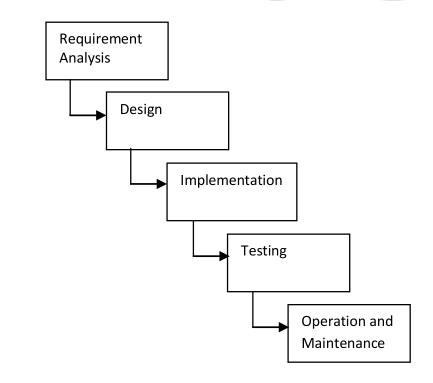
\includegraphics[scale=1]{Figs/Waterfall-Model}\\[1ex]
	\caption{Five phases of the waterfall Module ( \cite{Adenowo2013}).}
	\label{fig:waterfall}
\end{figure}

However, when projects run out of time, the testing phase will be cut, which may lead to poor quality outcomes. In addition, in the last step of implementation, developers may be unaware of steps they have taken; hence, it is impossible for developers to change the code until the last phase.

\begin{figure}[H]
	\centering    
	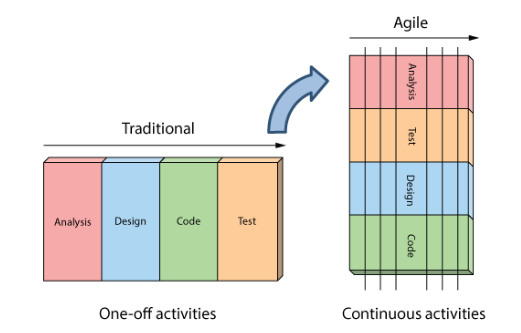
\includegraphics[scale=1]{Figs/Waterfull-Agile}\\[1ex]
	\caption{A comparison between Waterfall methodology and Agile methodology ( \cite{AgileVsWaterfall}).}
	\label{fig:waterfallAgile}
\end{figure}

Unlike with the Waterfall methodology which separates the whole project into several phases and implements it step by step, the Agile methodology separates the project into several tasks and every task is implemented in several phases. By doing this, it is changeable for developers when they find mistakes; therefore the quality and visibility issues of the Waterfall methodology are solved. For this reason, we adopt Agile as our guiding methodology when implementing this project.

\subsection{Project Timetable}

This section indicates time management for the project. This project can be separated into five phases  \cite{Laramee} as follow:

\begin{itemize}
	\item {1. }Requirements Specification; 
	Data Preprocessing; 
	Project Presentation;
	Exploring existing tools; 
	Project Specification; 
	complicated data processing techniques.
	\item {2. }Software Design;
	Candidate Classes and Responsibilities;
	Candidate Hierarchy;
	Collaboration and Subsystems;
	\item {3. }Implementation;
	Software Development;
	GUI;
	\item {4. }Debugging and Testing;
	\item {5. }Documentation;
\end{itemize}

Figure \ref{fig:gantterChart} indicates the Gantt chart of the project timeline. This project is initiated on the 17th February 2016, and the final deadline is the 15th December 2017. In every phase, there are several tasks to be done. Most of the tasks in phase one were completed by Dr. Tom Cheeseman before the data preprocessing took place; the second phase finished before July 2017, which allowed for more time to be used in the implementation phase. Priority needs to be given to software implementation, which will be executed according to the designs done by previous work. After the implementation, simple Graphic User Interface (GUI) framework will be put into effect. From the middle of November 2017, the project commenced its debugging and testing phase. Finally, a report and Doxygen was done in December 2017.
\begin{landscape}
	\begin{figure}[H]
		\centering    
		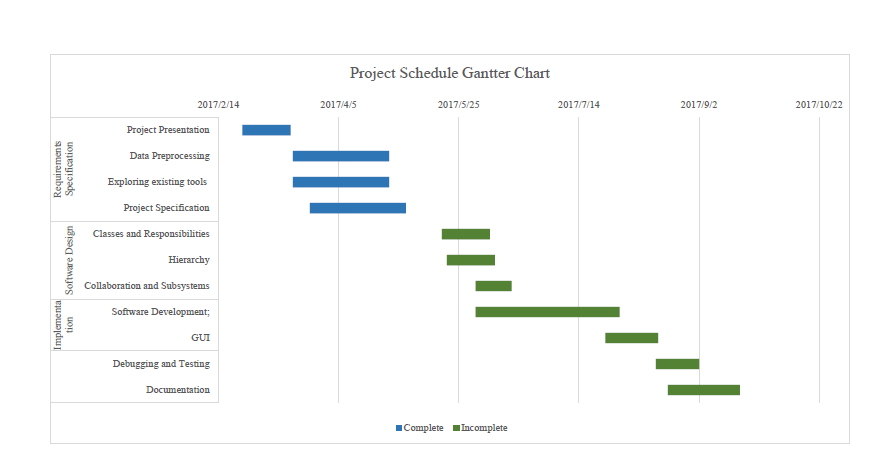
\includegraphics[scale=1]{Figs/Gantter-Chart}\\[1ex]
		\caption{Gantt chart for project timeline. }
		\label{fig:gantterChart}
	\end{figure}
	
\end{landscape}


\subsection{Risk Analysis}



This section explains the potential risks this project.
Figure \ref{fig:riskAnalysis} illustrates the analysis of these risks: The first risk is the limited time. The impact of limited time has been considered as high because the project requires a high level of attention to detail which is time-consuming. Regular meetings with the supervisor were important to consult on the difficulties encountered during the process. The second risk identified is the personal illness of the author. It is a low possibility risk with medium impact for the project. To deal with this case, keeping a good healthy is important to author herself. In addition, there is welfare service department on campus and the author has the international student’s insurance. Equipment failure is identified as the third risk. It is classified as medium in terms of both possibility and impacts. Yet the resources of  Swansea University are available 24 hours per day, which will reduce the impact of this risk. In addition, using the application Github for regular backup is essential. Data loss is considered as the fourth risk. The possibility of this happening is low but will cause high impact on the project. To avoid this situation, Dropbox is essential for backup. The last risk the necessities having a new supervisor, due to unforeseen circumstances. Swansea University procedure exists to support students by providing a second supervisor. 

\begin{figure}[H]
	\centering    
	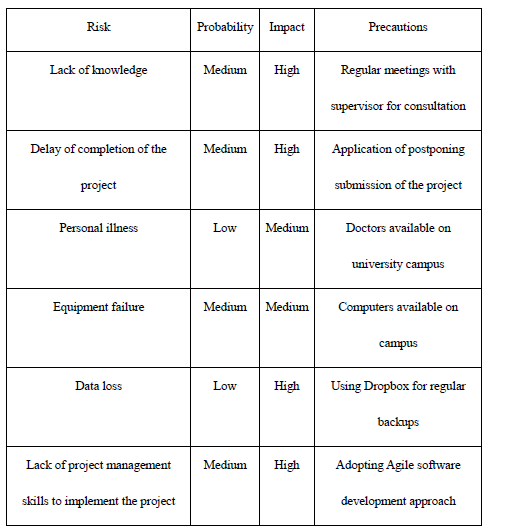
\includegraphics[scale=1]{Figs/Risk-Analysis}\\[1ex]
	\caption{A screenshot of Risk Analysis Table (\cite{Liu}). }
	\label{fig:riskAnalysis}
\end{figure}

